\documentclass[liststotoc,a4paper, 12pt]{scrartcl}
\usepackage[utf8]{inputenc}
\usepackage{ngerman}
\usepackage{setspace}
\usepackage{geometry}
\usepackage{graphicx}
\usepackage{cite}
\usepackage{listings}
\usepackage{color}


\geometry{a4paper, top=25mm, left=25mm, right=25mm, bottom=25mm}

\title{Bachelorarbeit}
\author{Kevin Seidel \\ Studiengang Informatik \\ Matrikelnummer: 943147}

\begin{document}
\begin{titlepage}
\begin{center}
	

\includegraphics[scale=0.1]{pictures/uos_logo.png}\\
\vspace*{1.5cm}
\begin{Large}
\textbf{Universität Osnabrück}
\end{Large}

\noindent\hrulefill
\\[0.25cm]
Fachbereich Informatik \\[3.5cm]
\begin{large}\textsc{Bachelorarbeit}\end{large} \\[2cm]
\begin{huge}\textbf{Indoor Positionierung mittels Bluetooth Low Energy} \end{huge} \\[1.5cm]
Erstellt am 28.01.2014
\\[3.5cm]
\textbf{Vorgelegt von:} \\
Kevin Seidel \\
Falkenstraße 43 \\
49124 Georgsmarienhütte \\
keseidel@uni-osnabrueck.de
\\[1cm]
\textbf{Geprüft von:} \\
Prof. Dr. Oliver Vornberger \\
Prof. Dr. Elke Pulvermüller

\end{center}
\end{titlepage}


\newpage

\pagenumbering{Roman}
\setcounter{page}{1}

\setcounter{secnumdepth}{-2}
\section*{Kurzfassung}%
\addcontentsline{toc}{section}{Kurzfassung}%

\newpage

\setuptoc{toc}{totoc}


\tableofcontents


\newpage

\listoffigures
\newpage

\listoftables
\newpage

\lstlistoflistings
\newpage

\pagenumbering{arabic}
\setcounter{page}{1}
\setcounter{secnumdepth}{2}


\section{Danksagung}

\section{Einleitung}
\subsection{Motivation}
Die GPS-Navigation ist seit Jahren aus keinem Auto mehr wegzudenken. Wo früher Karten genutzt wurden und nach Straßennamen geschaut wurde, wird heute die Zieladresse in das Navigationssystem eingegeben und das System bestimmt selbstständig die aktuelle Position, die Zielposition und errechnet die bestmögliche Route.
Ein Problem der GPS-Navigation ist jedoch, dass diese nur unter freiem Himmel akzeptabel funktioniert.
In der Realität verbringen wird jedoch den Großteil unserer Zeit in Gebäuden, wo uns dieser Ansatz wenig weiterhilft. 

Daher wäre es sinnvoll, eine Alternative zu GPS zu schaffen, welche diese Funktionien in Innenräume realisiert.
Da man jedoch für Innenräume kein eigenes Navigationssystem kaufen möchte, liegt die Idee nah, diese Konzept auf einem Gerät zu realisieren, was sowieso schon viele Leute besitzen und auch schon für die GPS-Navigation nutzen. 
Das Smartphone.
Wie in Abbildung 1 zu sehen, hat die Verbreitung der Smarthphones in den letzten Jahren sehr stark zugenommen, sodass man annehmen kann, das ein Großteil der potentiellen Nutzer der Indoor Positionierung auch ein Smartphoe besitzt.
\begin{figure}[htb]
	\centering
		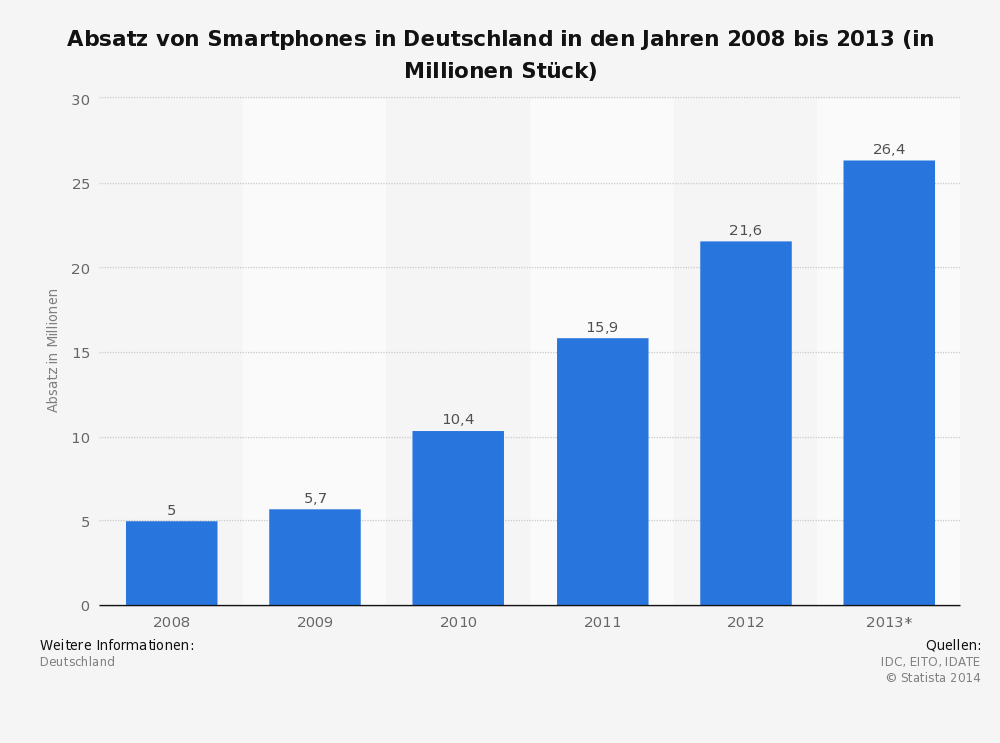
\includegraphics[height=8cm]{pictures/statistik-smartphonenutzung.png}
		\caption{Smartphoneabsatz in Deutschland}
\end{figure}

Für die Indoor Positionierung würden verschiedene Technologien in Frage kommen, wie zum Beispiel Wireless LAN, RFID oder Bluetooth.
Diese Technologien bieten sich an, da sie schon von Haus aus in vielen Smartphones integriert sind und so kein Bedarf an neuen Geräten oder Erweiterungen besteht.



Schlussendlich viel die Entscheidung der zu verwendenden Technologie auf Bluetooth, da dieses die höchste Verbreitung bietet und auch weitere Vorteile mit sich bringt. Zum einen ermöglicht Bluetooth eine schnelle und einfache Einrichtung und zum anderen benötigen die Bluetooth-Sendestationen nicht zwingend einen Stromanschluss, sondern erlauben auch einen Batteriebetrieb über mehrere Monate bis Jahre.

Die Positionierung in Innenräumen mittels Bluetooth ist ein relativ neuer Ansatz, welcher jedoch seit der Präsentation von Bluetooth Low Energy und der Vorstellung der iBeacons-Technologie von Apple immer mehr an Aufmerksamkeit gewonnen hat. 



\subsection{Ziele der Bachelorarbeit}
Das Hauptziel dieser Arbeit ist es zu untersuchen, in wie weit sich Bluetooth Low Energy beziehungsweise die darauf basierende iBeacons-Technologie für eine akzeptable Indoor Positionierung eignet, um Endgeräte zum Beispiel in Verkaufsräumen zu orten und zu identifizieren.


\section{Technologien}

\subsection{Bluetooth 4.0}
Die Bluetooth-Version 4.0, oder auch Bluetooth Smart genannt, wurde 2009 final spezifiziert und wird seit Ende 2010 in Endgeräten eingesetzt.
Dieser Standard beinhaltet neben dem klassischen Bluetooth, eine neue Version, mit dem Namen Bluetooth Low Energy, welche, wie der Name schon andeutet, einen sehr viel geringeren Stromverbrauch vorweißt. Dabei ist der Stromverbrauch zwischen zwei und 100 mal geringer als beim klassischen Bluetooth.

\subsubsection{Bluetooth Low Energy}
Bluetooth Low Energy wurde Anfangs von Nokia unter dem Namen ''Wibree'' entwickelt. Die Zielsetzung dabei war es eine Technologie zu entwickeln, mit der sich Computer und Mobilgeräte schnell und einfach mit Peripherie-Geräten verbinden lassen. Das Hauptaugenmerk galt dabei dem geringen Stromverbrauch, kompakter Bauweise und den Kosten für die benötigte Hardware.
Im Jahr 2007 wurden diese Spezifikationen dann in den, sich in der Entwicklung befindenden, Bluetooth-Standard 4.0 aufgenommen und daraufhin in Bluetooth Low Energy, oder kurz BLE umbenannt.

Bluetooth Low Energy arbeitet wie das klassische Bluetooth im 2,4 GHz Band, bringt aber in der Funktionsweise einige Unterschiede mit sich.

So wurde, im Vergleich zum klassischem Bluetooth, die Datenrate von bis zu 3 Mbit/s auf maximal 1 Mbit/s reduziert. Dies führt dazu, dass BLE zum Beispiel nicht für Headsets genutzt werden kann, da die zur Verffügung stehende Übertragungsrate nicht für die Audioübertragung ausreicht.

Die Vorteile die BLE mit sich bringt, liegen vor allem in der niedrigen Latenz, welche von 100ms auf bis zu unter 3ms reduziert wurde, und, wie bereits erwähnt, der Energieverbrauch drastisch gesenkt wurde.






\subsubsection{iBeacons}

\subsection{iOS und Xcode}

\subsection{CoreLocation-Framework}
\subsubsection{iBeacons-API}
\subsubsection{Weitere APIs}

\subsection{CoreData-Framework}


\section{Werkzeuge}
\subsection{Xcode}
\subsection{Versionsverwaltung mit Git}
\subsection{iPhone}

\section{Daten und Messungen}
\subsection{Mobile iBeacons}
\subsection{Stationäre iBeacons}
\subsection{Außenmessugen}
\subsection{Innenraummessungen}

\section{Umsetzung und Implementation}

\subsection{Ansatz zur Positionbestimmung}
\subsubsection{Trilateration}
\subsubsection{Fingerprinting}

\section{Fingerprinting}
\subsection{Positionbestimmung}
\subsubsection{Nearest-Neighbor-Verfahren}
\subsubsection{Probabilistisch-Verfahren}

\section{Fazit und Ausblick}

\section{Literatur}



\end{document}